\section{Combining stacks and the collimator}\label{sec:combine}

The engine blocks of Sec.~\ref{sec:megascale-remedies} need 32 to 64 rows, i.e.\ two to four 16-chip stacks of the kind described in Sec.~\ref{sec:rows}. A polarising beam splitter combines two stacks; we show here how to combine stacks in space with a slotted mirror at the collimator plane, and then repeat the analysis with the real, traced collimator. The second step changes little for the combiner, but it exposes a limit of the whole stacked relay: a cylindrical collimator at NA 0.9 defocuses the light of tweezers away from the row centre, so a row is usable over only half of its 180~\textmu m segment. We then design an all-reflective collimator that removes this limit. The record is \texttt{docs/\allowbreak megascale.md} (Secs.~11 to 13), \texttt{docs/\allowbreak collimator.md} (Sec.~10), \texttt{scripts/m26\_stack\_combine.py} and \texttt{scripts/m27\_reflective\_collimator.py}.

\subsection{A slotted comb at the collimator plane}\label{sec:combine-comb}

The plane S, formed by the back focal planes of the per-chip collimators, is conjugate to the atoms with magnification $1/D$. Here, $D=125$ for rows 4~\textmu m apart (Sec.~\ref{sec:rows}). At S, each chip's beam is a stripe of $\pm f_\mathrm{FAC}\mathrm{NA}_\mathrm{FAC}=\pm158$~\textmu m on the 0.5~mm chip pitch, so neighbouring beams leave gaps of 184~\textmu m. A mirror with slots, tilted at 45$^\circ$ (a ``comb''), placed in these gaps interleaves two stacks built at twice the chip pitch. Stack A passes through the slots; stack B, turned by 90$^\circ$, is reflected by the teeth. Each beam then sees a window of half-width $a\leq250$~\textmu m. The comb uses no polarisation, and the downstream relay is the same as for a single stack of all the rows. In addition, it doubles the chip pitch to 1.0~mm, which leaves room for the fibre and electrical access that the stacked relay left open (383 fast actuators per engine, 1,532 lines per four-engine chip).

Our choice of a 45$^\circ$ comb is a compromise between two considerations. First, it keeps the optical path of every row of stack B equal to that of stack A: with B's facets in the plane $y=-z_c$, the path to any plane $z=Z$ is $Z$ for all rows. However, the comb then spans the combined stack height along $z$, so the rows at the far end meet it farther from S, where the beams have spread. The question is therefore how far from S a window of half-width $a$ can sit.

\subsection{What sets the comb distance}\label{sec:combine-edge}

We propagate the field of one chip in $y$ from the collimator exit (aperture $f_\mathrm{FAC}$ before S, sine-condition lens, pupil fill $\beta=0.7$~\textmu m, $\mathrm{NA}_\mathrm{FAC}=0.9$) to the comb at a distance $z$ from S, apply the window, propagate back to S, and continue to the atoms through the pupil (\texttt{picsim/opa/stack.RelayY}, \texttt{results/\allowbreak m26\_edge.json}). Without a comb this reproduces the earlier stacked-relay values (transmission 0.973, crosstalk at 4~\textmu m $1.09\times10^{-4}$ against $1.06\times10^{-4}$). Table~\ref{tab:combine-edge} and Fig.~\ref{fig:combine-edge} give the penalty for a single tweezer.

\begin{table}[htbp]\centering\small
\caption{Comb penalty versus distance $z$ from S, single tweezer, 1D in $y$, ideal thin collimator with a hard edge, slot window of half-width $a$ (simulated, \texttt{results/\allowbreak m26\_edge.json}). Loss is the power clipped by the comb (\%); peak is relative to no comb; crosstalk (xt) to the neighbouring row at 4 and 3~\textmu m, in units of $10^{-4}$.}
\label{tab:combine-edge}
\begin{tabular}{lccccccc}
\toprule
 & \multicolumn{4}{c}{$a=250$~\textmu m} & \multicolumn{3}{c}{$a=225$~\textmu m} \\
$z$ from S & loss & peak & xt 4~\textmu m & xt 3~\textmu m & loss & peak & xt 4~\textmu m \\
\midrule
no comb & 0 & 1 & 1.1 & 2.9 & 0 & 1 & 1.1 \\
10~mm & $<0.1\%$ & 0.998 & 1.0 & 2.8 & 0.06\% & 0.992 & 1.1 \\
20~mm & 0.25\% & 0.992 & 1.5 & 4.0 & 0.72\% & 0.985 & 1.8 \\
30~mm & 0.85\% & 0.987 & 2.7 & 7.1 & 1.6\% & 0.981 & 3.1 \\
45~mm & 1.9\% & 0.973 & 6.0 & 17 & 3.4\% & 0.956 & 7.9 \\
60~mm & 3.6\% & 0.953 & 13 & 29 & 5.3\% & 0.931 & 16 \\
\bottomrule
\end{tabular}
\end{table}

\begin{figure}[htbp]\centering
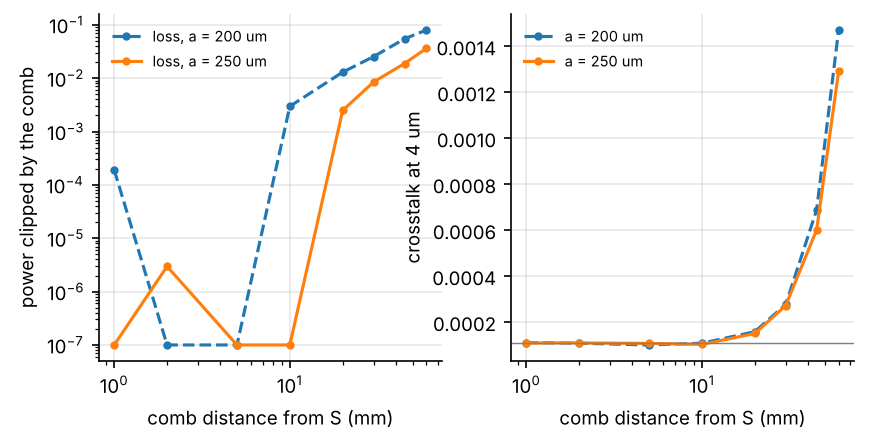
\includegraphics[width=0.8\linewidth]{m26_edge.png}
\caption{Comb penalty versus distance of the comb from S, single tweezer, 1D wave optics in $y$ (ideal thin sine-condition collimator, $\beta=0.7$~\textmu m, $\mathrm{NA}_\mathrm{FAC}=0.9$, hard edge, NA 0.5 pupil), for slot windows of half-width $a=200$~\textmu m (dashed) and 250~\textmu m (solid). Left: power clipped by the comb (values below $10^{-7}$ drawn at $10^{-7}$). Right: crosstalk to the neighbouring row at 4~\textmu m; grey line, without comb. The rise sets in near $z_\mathrm{max}=(a-f_\mathrm{FAC}\mathrm{NA}_\mathrm{FAC})D/\mathrm{NA}$.}
\label{fig:combine-edge}
\end{figure}

The hard edge of the collimator is not the problem. Its Fresnel tail spreads into the gap, but it consists of directions steeper than the pupil accepts, and clipping it costs nothing. A Fresnel-tail estimate that ignores the pupil predicts 0.36\% loss at 10~mm; the simulated loss there is below 0.1\%. A graded collimator edge (raised cosine from 0.8 to 0.9 of the aperture) therefore does not help: it raises the baseline crosstalk to $1.5\times10^{-4}$ and gains no distance. What matters is the light inside the pupil acceptance, which leaves S at half-angle $\mathrm{NA}/D=4$~mrad. It reaches the window edge at
\begin{equation}
z_\mathrm{max}=\frac{(a-f_\mathrm{FAC}\mathrm{NA}_\mathrm{FAC})\,D}{\mathrm{NA}},
\label{eq:zmax}
\end{equation}
which is 23~mm for $a=250$~\textmu m and 17~mm for $a=225$~\textmu m. This agrees with the scan: at $z=20$~mm and $a=250$~\textmu m the worst row loses 0.25\% and the crosstalk at 4~\textmu m rises from $1.1\times10^{-4}$ to $1.5\times10^{-4}$, while at 30~mm it reaches $2.7\times10^{-4}$. A single edge, as used for block combining (rows 0 to 15 from one stack and 16 to 31 from the other), behaves similarly. It also shifts the boundary row by 1.7~nm at $z=20$~mm ($a=250$~\textmu m) and by 12~nm at $a=200$~\textmu m, a static offset to calibrate. The rows are mutually incoherent (\texttt{docs/\allowbreak row\_coherence.md}), so this crosstalk adds in intensity.

\subsection{Layouts for 32 to 64 rows}\label{sec:combine-layouts}

Table~\ref{tab:combine-layout} lists the layouts (\texttt{results/\allowbreak m26\_layout.json}). We place the first comb point at $z_c=7.0$~mm, 0.5~mm (a choice) beyond the $x$ slit plane of the traced $x$ lens and collimator (Sec.~\ref{sec:combine-lens}), and the worst row is the one at the far end of the comb. Two 16-chip stacks at 1.0~mm pitch need a comb from 7 to 23~mm, which ends at $z_\mathrm{max}$; their worst row loses 0.45\% of its power, with peak 0.991 and crosstalk $1.8\times10^{-4}$ at 4~\textmu m. Two such pairs, combined by a polarising beam splitter (PBS), give 64 rows at the same penalty. Combining only by comb with longer stacks puts the far rows beyond $z_\mathrm{max}$ (7 to 31~mm for 24-chip stacks, 7 to 39~mm for 32-chip stacks) and costs up to 1.3\% and $3.9\times10^{-4}$. A second comb level (stacks at 2.0~mm, combined pairwise and then again) would put the second comb beyond $z_\mathrm{max}$, so we do not use it. With $a=225$~\textmu m, which is about what a 50~\textmu m tooth plate ($t/(2\sqrt{2})=18$~\textmu m per edge) and $\pm10$~\textmu m edge placement leave, the worst rows of the two preferred layouts lose 0.86\% and reach $2.0\times10^{-4}$.

\begin{table}[htbp]\centering\small
\caption{Layouts for 32 to 64 rows (simulated and derived, \texttt{results/\allowbreak m26\_layout.json}; first comb point at $z_c=7$~mm). Worst row at $a=250$~\textmu m: power loss, peak and crosstalk at 4~\textmu m (units of $10^{-4}$). The last column states whether the objective must accept both polarisations. Bold: preferred layouts.}
\label{tab:combine-layout}
\setlength{\tabcolsep}{4pt}
\begin{tabular}{lllccccc}
\toprule
 & & chips per & comb & \multicolumn{3}{c}{worst row} & pol.-insensitive \\
rows & layout & stack, pitch & $z$ range & loss & peak & xt 4~\textmu m & objective \\
\midrule
32 & one stack & 32, 0.5~mm & & \multicolumn{3}{c}{(no comb)} & no \\
32 & 2 stacks, PBS & 16, 0.5~mm & & \multicolumn{3}{c}{(no comb)} & yes \\
32 & \textbf{2 stacks, comb} & \textbf{16, 1.0~mm} & \textbf{7--23~mm} & \textbf{0.45\%} & \textbf{0.991} & \textbf{1.8} & \textbf{no} \\
48 & 4 stacks, comb + PBS & 12, 1.0~mm & 7--19~mm & 0.21\% & 0.992 & 1.4 & yes \\
48 & 2 stacks, comb & 24, 1.0~mm & 7--31~mm & 0.93\% & 0.987 & 2.9 & no \\
64 & \textbf{4 stacks, comb + PBS} & \textbf{16, 1.0~mm} & \textbf{7--23~mm} & \textbf{0.45\%} & \textbf{0.991} & \textbf{1.8} & \textbf{yes} \\
64 & 2 stacks, comb & 32, 1.0~mm & 7--39~mm & 1.3\% & 0.984 & 3.9 & no \\
64 & 2 stacks, PBS & 32, 0.5~mm & & \multicolumn{3}{c}{(no comb)} & yes \\
\bottomrule
\end{tabular}
\end{table}

A single taller stack (32 or 64 chips at 0.5~mm) needs no combiner. In first-order optics it only enlarges the $y$-relay field, to $\pm8$ or $\pm16$~mm at the first telescope lens and 3.7 or 7.4~mrad at the pupil. Its costs are mechanical: 16 to 32~mm of facets flush to about 100~\textmu m, and all the input and output lines at 0.5~mm pitch.

\paragraph{2D check.} The 1D model leaves out the circular pupil, which couples $x$ and $y$, and the full rows. We therefore pass the comb-windowed $y$ pupil of both chips through the 2D model of the stacked relay (D1 $x$ response, circular NA 0.5 pupil; \texttt{results/\allowbreak m26\_twod.json}). Chip $m$ forms a full row of 41 tweezers at 3~\textmu m, chip $m+1$ forms 11 tweezers offset by 1.5~\textmu m, and one tweezer of chip $m$ then moves by 0.25~\textmu m. Without a comb this reproduces the earlier 2D values. Table~\ref{tab:combine-2d} shows that 2D does not change the conclusions. At the worst row the full-row crosstalk rises by a factor 1.3, and the effect of a moving tweezer on the next row by a factor 1.55 to 1.65 (to $3.9\times10^{-5}$ in depth at 4~\textmu m, $9.6\times10^{-5}$ at 3~\textmu m). This is still more than an order of magnitude below the in-row figures of D1 (0.11\%, 3.5~nm). Tweezers at $x=0$ and at the row end (60~\textmu m) give the same values to 0.1\%, because the comb acts on $y$ alone and the circular pupil couples the two axes only weakly. The 1D single-tweezer crosstalk ($1.8\times10^{-4}$ at $z=23$~mm) slightly overstated the 2D one ($1.5\times10^{-4}$). The block-combining edge moves the boundary row by 7~nm in 2D (peak position), a static offset to calibrate. With coherent rows the comb would raise the static depth change at 4~\textmu m from 2.6\% to 2.9\%; rows must stay incoherent, as they must without a comb.

\begin{table}[htbp]\centering\small
\caption{2D check of the comb (simulated, \texttt{results/\allowbreak m26\_twod.json}; both chips windowed, rows incoherent). Crosstalk (xt) and the relative change of the neighbour row's trap depth in units of $10^{-4}$; neighbour row at 4~\textmu m, at 3~\textmu m in brackets.}
\label{tab:combine-2d}
\setlength{\tabcolsep}{4pt}
\begin{tabular}{lccccc}
\toprule
 & \multicolumn{2}{c}{single tweezer} & full row & \multicolumn{2}{c}{neighbour depth change} \\
comb & peak & xt 4~\textmu m & xt 4~\textmu m, max over $x$ & static & moving tweezer \\
\midrule
none & 1 & 1.1 & 1.8 & 1.7 (2.0) & 0.24 (0.62) \\
$z$ 15~mm, $a$ 250~\textmu m & 0.995 & 1.1 & 1.8 & 1.8 (2.2) & 0.29 (0.74) \\
$z$ 23~mm, $a$ 250~\textmu m (worst row) & 0.990 & 1.5 & 2.3 & 2.1 (2.6) & 0.39 (0.96) \\
$z$ 23~mm, $a$ 225~\textmu m & 0.982 & 1.6 & 2.4 & 2.2 (2.2) & 0.39 (0.80) \\
$z$ 30~mm, $a$ 250~\textmu m ($>z_\mathrm{max}$) & 0.984 & 2.1 & 2.9 & 2.5 (3.1) & 0.53 (1.2) \\
single edge, $z$ 23~mm, $a$ 250~\textmu m & 0.995 & 1.3 & 2.0 & 1.9 (2.2) & 0.34 (0.84) \\
\bottomrule
\end{tabular}
\end{table}

\paragraph{Tolerances.} The tolerances follow from the conjugations and the decentre results of the stacked relay (derived). A comb tilt $\theta$ about $x$ deflects stack B by $2\theta$ at S. This shifts its facet image in the pupil by $2\theta F_y$, with $F_y=2.17$~m, which gives 1\% peak loss at $\theta=0.16$~mrad and 3\% at 0.28~mrad. The same tilt moves B's rows by $2\theta z/D$: 0.32~nm per \textmu rad at $z=20$~mm, and 50~nm at 0.16~mrad. This static offset alternates between rows, because A and B rows interleave, so it must be calibrated once against the static array; keeping the alternating pitch error below 3~nm then needs a tilt stability of about 10~\textmu rad (drift, not alignment; mount stability not yet checked against a source [REF?]). Moving the comb by $\mathrm{d}z$ along $z$ changes B's path by $\mathrm{d}z$, which tolerates 100~\textmu m (chip piston, peak $\geq0.992$); it also shifts the windows by $\mathrm{d}z$ in $y$, which should stay within about $\pm10$~\textmu m. Light that misses a tooth leaves at 90$^\circ$ to a dump; light from stack A that hits the back of a tooth is reflected towards stack B and needs an absorbing back face.

\paragraph{Comb roll.} A comb edge that is not parallel to $x$ makes the window depend on $x$. Beyond the slit plane the $x$ relay is telecentric, so each tweezer meets the comb at its slit-plane position $X=f_1 s$, and four engines at 3.0~mm pitch span $X=\pm5.6$~mm. One tweezer's footprint at the comb is at most $\pm0.78$~mm (17~mm beyond the slit plane, half-angle $(A/2)/f_1=0.046$). Hence, for a roll of 2~mrad, the edge moves by only 3~\textmu m across one tweezer, against the tens of \textmu m over which the result changes, and we treat each tweezer with its local window $a(X)$. In 2D at $z=23$~mm the peak falls from 0.989 to 0.972 as $a$ goes from 250 to 205~\textmu m (about 0.04\% per \textmu m), while the crosstalk at 4~\textmu m stays at 1.4 to $1.6\times10^{-4}$. A roll therefore mainly makes the depth vary along the row, by about $\pm0.4\%$ for a $\pm10$~\textmu m change of $a$, which a 1.8~mrad roll produces over $\pm5.6$~mm. The engines set each tweezer's power in any case, so this is a calibration, not a limit; the same holds for an edge straightness of $\pm10$~\textmu m over 12~mm.

Thus the blocks of Sec.~\ref{sec:megascale} can be built as follows. (i) For 32 rows, two 16-chip stacks at 1.0~mm pitch and one comb. This needs no polarisation optics, and since alternate rows come from different stacks, the passive orthogonal-polarisation decorrelation of \texttt{docs/\allowbreak row\_coherence.md} comes for free if the objective accepts it. (ii) For 64 rows, two such comb pairs combined by a PBS. Four 16-chip stacks with four engines per chip at 3.0~mm pitch (12~mm edge) then form the 64~$\times$~4 block, with 256 engines and 98,048 fast actuators. With intermediate steps at $10^6$ sites it reaches a time average of $2.9\times10^{-4}$ on 4~$\times$~4~\textmu m and $2.7\times10^{-4}$ on 3~$\times$~4~\textmu m, without the 24~mm chip edge that 32~$\times$~8 needs. The worst rows lose 0.9 to 1.5\% of their peak depth to the comb ($a=250$ / 225~\textmu m), which the per-tweezer power set by the engines recovers. The edge scan is 1D in $y$ and the 2D check uses the same windowed pupil; both take the window of each slot at one distance $z$, whereas the 45$^\circ$ tilt places the two edges of a 0.5~mm slot 0.25~mm before and after that distance, which changes $z$ by at most 4\% at $z_c=7$~mm. Tooth-edge roughness, scatter from the comb and a lens design of the larger $y$-relay field are not included.

\subsection{The comb with the real collimator}\label{sec:combine-lens}

The analysis above used an ideal thin collimator in air. The adopted collimator is a fused-silica Weierstrass block glued to the facet, followed by a 10~\textmu m gap and a 250~\textmu m aplanat of index 1.8 (\texttt{docs/\allowbreak collimator.md}). We repeat the comb study with this traced lens (\texttt{results/\allowbreak m26\_lens.json}). The exit field is built from the traced lens map (exit height, wavefront and amplitude per ray) at a plane 60~\textmu m beyond the last vertex, and S lies at the traced back focal plane, 0.44~mm from the facet. Without a comb this reproduces the wave model of the traced collimator: crosstalk $8.0\times10^{-5}$ at 4~\textmu m against $8.4\times10^{-5}$, and $3.8\times10^{-4}$ against $4.0\times10^{-4}$ at 3~\textmu m. The real geometry also moves the comb. The traced $x$ lens puts the $x$ slit plane 6.76~mm from the facet, the collimator glass adds 0.15~mm in $x$ ($t(1-1/n)$ per section), and we keep 0.5~mm of clearance; the comb therefore starts 7.0~mm from S, and the far row of a 32-row comb sits at 23.0~mm.

\begin{table}[htbp]\centering\small
\caption{Comb penalty with the real (traced) collimator against the ideal thin collimator, slot window $a=250$~\textmu m, 1D (simulated, \texttt{results/\allowbreak m26\_lens.json}). Values for $a=225$~\textmu m are given in the text.}
\label{tab:combine-lens}
\setlength{\tabcolsep}{4pt}
\begin{tabular}{lcccccc}
\toprule
 & \multicolumn{3}{c}{real collimator} & \multicolumn{3}{c}{thin collimator} \\
$z$ from S & loss & peak & xt 4~\textmu m & loss & peak & xt 4~\textmu m \\
\midrule
15~mm & $5\times10^{-4}$ & 0.994 & $7.6\times10^{-5}$ & $5\times10^{-4}$ & 0.994 & $1.2\times10^{-4}$ \\
20~mm & $2.6\times10^{-3}$ & 0.991 & $9.2\times10^{-5}$ & $2.5\times10^{-3}$ & 0.992 & $1.5\times10^{-4}$ \\
23.0~mm (far row) & $5.0\times10^{-3}$ & 0.991 & $1.1\times10^{-4}$ & $4.5\times10^{-3}$ & 0.991 & $1.8\times10^{-4}$ \\
30~mm & $9.0\times10^{-3}$ & 0.988 & $1.9\times10^{-4}$ & $8.5\times10^{-3}$ & 0.987 & $2.7\times10^{-4}$ \\
\bottomrule
\end{tabular}
\end{table}

As can be seen from Table~\ref{tab:combine-lens}, the immersed facet puts more light near the edge of the beam at S, but loss and peak follow the thin-lens values within 12\%, and the crosstalk is lower. With $a=225$~\textmu m the real collimator gives loss / peak / crosstalk at 4~\textmu m of $3.4\times10^{-3}$ / 0.986 / $7.5\times10^{-5}$ at 15~mm, $7.6\times10^{-3}$ / 0.985 / $9.7\times10^{-5}$ at 20~mm, $9.3\times10^{-3}$ / 0.986 / $1.2\times10^{-4}$ at the far row and $1.7\times10^{-2}$ / 0.983 / $2.0\times10^{-4}$ at 30~mm. Equation~\eqref{eq:zmax} therefore still holds. In 2D at the far row ($z=23.0$~mm, $a=250$~\textmu m), the full-row crosstalk at 4~\textmu m is $1.6\times10^{-4}$ ($1.75\times10^{-4}$ without the comb). A moving tweezer changes the next row by $2.8\times10^{-5}$ in depth at 4~\textmu m ($1.2\times10^{-5}$ without the comb) and by $6.9\times10^{-5}$ at 3~\textmu m ($3.6\times10^{-5}$). Hence the comb conclusions hold for the real collimator in the real geometry.

\subsection{Skew rays: light that leaves the chip at an angle along \texorpdfstring{$x$}{x}}\label{sec:combine-skew}

A tweezer at position $x_a$ along the row is formed by light that leaves the emitters with $x$ direction sine $s_x=x_a/x_\mathrm{scale}$. Here, $x_\mathrm{scale}=288$~\textmu m for D1, so $s_x$ reaches 0.31 at the end of a 180~\textmu m segment and 0.355 at the slit edge. The collimator is cylindrical: its surface normals have no $x$ component, so $k_x$ is conserved, and the $y$-$z$ problem is exactly the 2D trace with every index $n$ replaced by the effective index
\begin{equation}
n_\mathrm{eff}=\sqrt{n^2-s_x^2}.
\end{equation}
A unit test checks this against 3D vector refraction. All earlier $y$ models (the stacked relay, the traced collimator, and the comb study above) used $s_x=0$. For $s_x>0$ the effective index ratios of the lens rise, from 1.45 to 1.50 for the block and from 1.80 to 1.89 for the aplanat at $s_x=0.355$, and the lens is no longer aplanatic for the facet (\texttt{results/\allowbreak m26\_skew.json}). Table~\ref{tab:combine-skew} and Fig.~\ref{fig:combine-skew} give the result.

\begin{table}[htbp]\centering\small
\caption{Tweezer at $x_a$ with the adopted collimator, relative to an ideal collimator at the same $s_x$ (simulated, \texttt{results/\allowbreak m26\_skew.json}; effective-index trace, downstream relay ideal, no comb; with the comb at the far row the crosstalk changes by a factor 0.9 to 1.6). Peak in 1D (2D in brackets), equivalent facet focus error, residual wavefront after refocusing the facet for this tweezer, and crosstalk at 4~\textmu m.}
\label{tab:combine-skew}
\begin{tabular}{lcccc}
\toprule
$x_a$ ($s_x$) & peak & equivalent facet defocus & residual after refocusing & xt 4~\textmu m \\
\midrule
0 & 1.000 (1.000) & 0 & 0 & $8.4\times10^{-5}$ \\
15~\textmu m (0.052) & 0.999 (0.997) & $-0.27$~\textmu m & 0.001 waves & $2.2\times10^{-4}$ \\
30~\textmu m (0.104) & 0.971 (0.942) & $-1.10$~\textmu m & 0.005 waves & $3.0\times10^{-3}$ \\
45~\textmu m (0.156) & 0.794 (0.725) & $-2.46$~\textmu m & 0.014 waves & $8.2\times10^{-3}$ \\
60~\textmu m (0.208) & 0.481 (0.440) & $-4.36$~\textmu m & 0.029 waves & $6.9\times10^{-3}$ \\
90~\textmu m (0.312) & 0.231 & $-9.67$~\textmu m & 0.096 waves & $9.0\times10^{-3}$ \\
\bottomrule
\end{tabular}
\end{table}

\begin{figure}[htbp]\centering
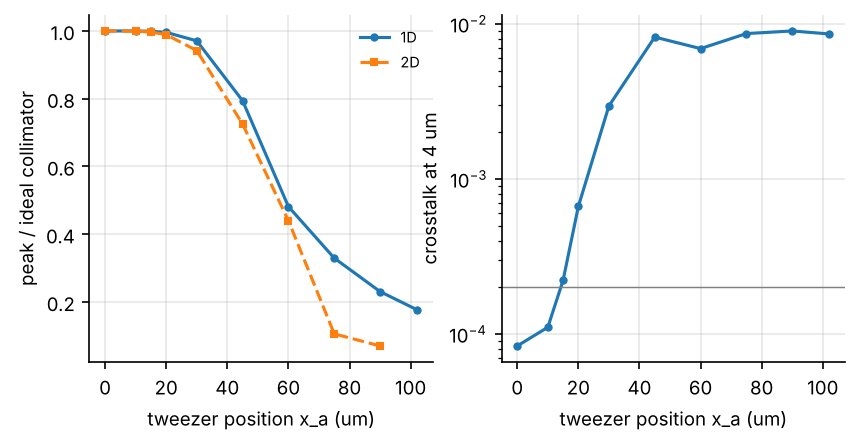
\includegraphics[width=0.8\linewidth]{m26_skew.png}
\caption{Effect of the $x$ direction sine $s_x=x_a/288$~\textmu m on the adopted cylindrical collimator (glued fused-silica Weierstrass block and 250~\textmu m aplanat of index 1.8, NA 0.9), traced with effective indices $\sqrt{n^2-s_x^2}$, with an ideal downstream relay, no comb and no facet focus offset. Left: peak of a tweezer at $x_a$ relative to an ideal collimator at the same $s_x$, 1D (solid) and 2D with the circular NA 0.5 pupil (dashed). Right: crosstalk at 4~\textmu m to the neighbouring row (1D); grey line at $2\times10^{-4}$ for reference.}
\label{fig:combine-skew}
\end{figure}

The error is almost purely a focus shift of the facet,
\begin{equation}
\Delta z\approx-99\,s_x^2~\text{\textmu m}.
\end{equation}
A thin glass lens in air would give $-f(n+1)s_x^2/(2n)=-148\,s_x^2$~\textmu m, the same order. Refocusing the facet for one tweezer restores its peak fully; the residual after refocusing stays below 0.1 waves up to 90~\textmu m. However, all tweezers of a row share the facet and the collimator. The phase error sits at S, which is conjugate to the atoms, so refocusing the atom plane does not help either. In 2D the best atom-plane focus recovers the peak up to $x_a=30$~\textmu m (1.02), but with a 1.5~\textmu m $y$-focus shift, outside the $\pm0.5$~\textmu m axial registration of the transport model (Sec.~\ref{sec:transport}), and not beyond. The 2D model covers $|x_a|\leq60$~\textmu m only: its engine (D1, 128 ports) cannot form a tweezer beyond about 67~\textmu m for any collimator.\footnote{An earlier version read the 2D values at 75 and 90~\textmu m (peak 0.11 at 75~\textmu m) as a break-up of the spot in the circular pupil. They are outside the model; the 1D results, which do not involve the engine, hold to the slit edge.}

\paragraph{What a common focus offset recovers.} A single facet offset for the whole row, i.e.\ the length of the glued block set at fabrication, trades the centre against the ends (\texttt{results/\allowbreak m26\_skew\_offset.json}, first-order focus phase, 1D). With $\Delta z=-1.25$~\textmu m the peak stays at or above 0.96 out to $|x_a|=45$~\textmu m, and the static crosstalk at 4~\textmu m stays at or below $3.6\times10^{-3}$. That is within the criteria of \texttt{docs/\allowbreak row\_coherence.md} (others' depth change below $3\times10^{-3}$ when a tweezer moves), since for incoherent rows the moving-tweezer effect was about 0.13 of the static crosstalk in the earlier stacked-relay model; we did not recompute it for skewed tweezers. Beyond 50~\textmu m no offset helps: the peak is 0.90 at 50~\textmu m and 0.66 at 60~\textmu m, and no offset brings the worst peak over $|x_a|\leq90$~\textmu m above 0.43.

\paragraph{Consequences.} A refractive cylindrical collimator at NA 0.9 serves about half of the 180~\textmu m segment ($|x_a|\leq45$~\textmu m, about 23 sites at 4~\textmu m), not all of it. Every power and crosstalk figure of the stacked relay, of the traced collimator and of the comb study above holds near the row centre and is optimistic for the outer half. For the large arrays of Sec.~\ref{sec:megascale} this doubles the number of engines per row at fixed coverage (90~\textmu m segments instead of 180~\textmu m). The alternative is a collimator that is insensitive to $s_x$. Serving $|x_a|\leq90$~\textmu m within the $\pm0.5$~\textmu m focus tolerance, with the best common offset, needs $|\Delta z/s_x^2|\leq10$~\textmu m, ten times less than now. The all-reflective collimator of Sec.~\ref{sec:combine-reflective} meets this with $\Delta z=0$.

We see four routes. (i) An all-reflective collimator in one medium. The law of reflection and a uniform medium are unchanged by the effective-index map, so the wavefront error vanishes for every $s_x$, and a flat exit face normal to the collimated beam keeps it so (derived). It needs a folded geometry within the 0.5~mm chip pitch; we design it in Sec.~\ref{sec:combine-reflective}. (ii) A cemented refractive design. Glass-glass interfaces are less sensitive than glass-air ones (relative power change $0.41\,s_x^2$ for a 1.45 to 2.0 interface against $0.84\,s_x^2$ for 1.45 to air, derived), but a factor of two is not enough on its own. (iii) A corrector at the $x$ slit plane, where $x$ encodes $s_x$. This fails at large $s_x$: at $x_a=90$~\textmu m the error acts at S like a $y$ lens of 4~mm focal length (2.9 waves at 158~\textmu m), so the beam has passed a focus before it reaches the slit plane, 6.5~mm later. (iv) A larger vertical facet mode, i.e.\ a lower facet NA. This helps by less than a factor of two, because the optimal pupil fill, and with it $f_\mathrm{FAC}$, grows with the mode. Of these, only the reflective route removes the error in principle. The downstream cylindrical lenses of the $y$ relay see $x$ angles below about 0.05 and are not modelled; the skew trace is exact for cylindrical surfaces, but the downstream relay is taken as ideal, and the common-offset result uses a first-order focus phase in 1D.

\subsection{An all-reflective collimator}\label{sec:combine-reflective}

\paragraph{Why two mirrors.} A mirror in one medium keeps the wavefront flat at every $s_x$, as argued above. One mirror (an off-axis parabola) collimates, but maps the far field with a strongly asymmetric distortion for a cone of $\pm38^\circ$ in glass. Two mirrors designed together can meet two conditions, exact collimation and the sine condition in the medium, $y_S-y_c=\pm nf\sin\theta$. Here, $\theta$ is the ray angle in the glass, $y_c$ the centre of the collimated beam and $f=175$~\textmu m. Under the effective-index map such a pair stays aplanatic. Only its focal length changes, to $fn/n_\mathrm{eff}$, i.e.\ by 3.1\% at the slit edge in fused silica (7\% in air). The stripe edge at S does not move, because the rim of the first mirror fixes $\theta$ (derived).

\paragraph{Construction and selection.} We construct the pair as the refractive aplanat of Sec.~\ref{sec:rows-collimator} is constructed (Wassermann-Wolf in 2D), with mirrors. The first mirror M1 is $r(\theta)(\sin\theta,\cos\theta)$ from the facet. The direction after M1 follows in closed form from a constant optical path to a plane, the law of reflection gives $r'=r\cot[(\phi-\theta)/2]$, and the second mirror M2 then sends every ray along $z$ (\texttt{picsim/\allowbreak opa/\allowbreak mirror\_collimator.py}). We scanned 3,780 constructions over the distance of M1, the beam centre, the fold angle and the mapping orientation (\texttt{results/\allowbreak m27\_scan.json}). We kept those with no light behind the facet plane, no obscuration, a radius of curvature of at least 20~\textmu m, and no overlap between the blocks of neighbouring chips at 0.5~mm pitch, with 10~\textmu m clearance around each block's light. 290 layouts pass. A normal displacement $\delta$ of a back-surface mirror in glass changes the path by $2n\cos i\,\delta$. Over the passing layouts this sensitivity is 2.1 to 3.2, rms over the pupil (against 0.45 to 0.8 for a refracting surface of the adopted design), and grazing folds are the least sensitive but the longest. We adopted the least sensitive layout no longer than 0.5~mm, a choice comparable to the 0.40~mm refractive collimator.

\begin{table}[htbp]\centering\small
\caption{Adopted all-reflective collimator (simulated, \texttt{results/\allowbreak m27\_scan.json}, \texttt{m27\_trace.json}, \texttt{m27\_wave.json}, \texttt{m27\_tolerance.json}). Fused silica ($n=1.4496$) glued to the facet; $f=175$~\textmu m, NA~0.9; on-axis wave-model figures at $\beta=0.7$~\textmu m.}
\label{tab:combine-refl}
\begin{tabular}{ll}
\toprule
quantity & value \\
\midrule
M1 distance on axis / beam centre / axial fold & 50~\textmu m / $-390$~\textmu m / $-70^\circ$ \\
block length (facet to exit face) / glass path of the axial ray & 476~\textmu m / 749~\textmu m \\
$y$ extent of the light / largest cross-section & $-547$ to $+17$~\textmu m / 315~\textmu m \\
incidence on M1 / on M2 (critical angle $43.6^\circ$) & $28$ to $77^\circ$ / $44.6$ to $60.0^\circ$ (TIR) \\
smallest radius of curvature, M1 / M2 & 193 / 798~\textmu m \\
wavefront, 3D trace, $s_x\leq0.355$ & $<2\times10^{-12}$ waves p-v \\
peak per guided power / $y$ FWHM / crosstalk at 4~\textmu m ($s_x=0$) & 1.10 / 1.35~\textmu m / $8\times10^{-5}$ \\
mirror-pair reflectance, M1 silver / gold, M2 TIR & 0.996 / 0.982 \\
laser power per 1.2~mK tweezer, M1 silver & 57.7~mW \\
facet decentre / focus for $\leq3\%$ loss & $\pm0.1$ / $\pm1$~\textmu m \\
mirror form error for $\leq2\%$ loss & $\leq10$~nm rms \\
\bottomrule
\end{tabular}
\end{table}

\begin{figure}[htbp]\centering
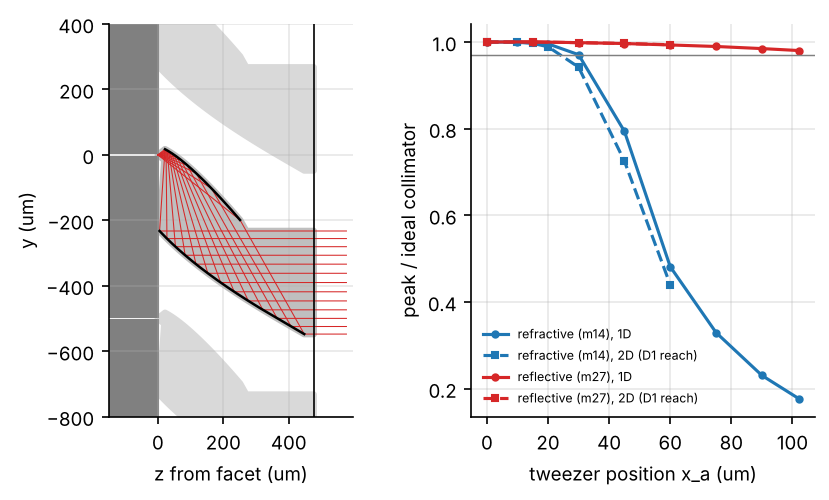
\includegraphics[width=0.95\linewidth]{m27_figure.png}
\caption{Left: $y$-$z$ section of the adopted all-reflective collimator, from the facet (origin) to the flat exit face (vertical line), with rays every $6.4^\circ$ in the glass; mirrors in black. Grey: light regions, with 10~\textmu m margin, of the blocks of the neighbouring chips at $\pm0.5$~mm; dark grey: the chips ($z<0$). Right: peak of a tweezer at $x_a$ relative to an ideal collimator at the same $s_x$ (effective-index trace, verified by a 3D vector trace; downstream relay ideal), for the refractive collimator of Sec.~\ref{sec:combine-skew} (blue) and the reflective one (red); 1D to the slit edge, 2D only within the 67~\textmu m reach of the D1 engine of the 2D model.}
\label{fig:combine-refl}
\end{figure}

\paragraph{Exactness.} We traced the adopted design independently, in 3D, with rays launched with $k_x$ (not with the effective index), the vector law of reflection on spline fits of the two mirror curves, and the optical path as $n$ times the 3D length (\texttt{results/\allowbreak m27\_trace.json}). At $s_x=0$, 0.1, 0.2, 0.312 and 0.355 the phase of the $k_x=k_0s_x$ component is flat to $2\times10^{-12}$ waves, the exit height equals $fs\,n/n_\mathrm{eff}$ to $2\times10^{-10}$, and the 2D effective-index lens map used by the wave model agrees with the 3D trace. The refractive collimator carries 0.30, 1.18, 2.86 and 3.67 waves p-v at the same $s_x$.

\paragraph{Performance.} On axis the reflective collimator equals the refractive one to four digits in the wave model (\texttt{results/\allowbreak m27\_wave.json}). Across the row it holds the peak and the crosstalk (Table~\ref{tab:combine-refl-skew}, Fig.~\ref{fig:combine-refl}; \texttt{results/\allowbreak m27\_skew.json}). The remaining 1.5\% at 90~\textmu m is the 2.4\% longer focal length; relative to its own centre the tweezer keeps 0.990. The $y$ centroid does not move, because the mapping stays antisymmetric. Hence one engine serves its whole 180~\textmu m segment without a common focus offset, and the doubling of engines discussed above is not needed.

\begin{table}[htbp]\centering\small
\caption{Tweezer at $x_a$ with the reflective and the refractive collimator, relative to an ideal collimator at the same $s_x$ (simulated, \texttt{results/\allowbreak m27\_skew.json} and \texttt{m26\_skew.json}). Peak in 1D (2D in brackets, within the reach of the D1 engine), crosstalk at 4~\textmu m, and the loss of the comb at the far row of a 32-row block ($a=250$~\textmu m, 23.5~mm from S for the reflective design).}
\label{tab:combine-refl-skew}
\setlength{\tabcolsep}{4pt}
\begin{tabular}{lccccc}
\toprule
 & \multicolumn{2}{c}{peak} & \multicolumn{2}{c}{xt 4~\textmu m} & comb loss \\
$x_a$ & reflective & refractive & reflective & refractive & reflective \\
\midrule
0 & 1.000 (1.000) & 1.000 (1.000) & $8.4\times10^{-5}$ & $8.4\times10^{-5}$ & $4.8\times10^{-3}$ \\
30~\textmu m & 0.999 (0.999) & 0.971 (0.942) & $8.4\times10^{-5}$ & $3.0\times10^{-3}$ & $4.9\times10^{-3}$ \\
45~\textmu m & 0.997 (0.997) & 0.794 (0.725) & $8.6\times10^{-5}$ & $8.2\times10^{-3}$ & $5.0\times10^{-3}$ \\
60~\textmu m & 0.993 (0.994) & 0.481 (0.440) & $9.0\times10^{-5}$ & $6.9\times10^{-3}$ & $5.1\times10^{-3}$ \\
90~\textmu m & 0.985 & 0.231 & $9.7\times10^{-5}$ & $9.0\times10^{-3}$ & $5.4\times10^{-3}$ \\
102~\textmu m (slit edge) & 0.980 & 0.177 & $1.0\times10^{-4}$ & $8.6\times10^{-3}$ & $5.5\times10^{-3}$ \\
\bottomrule
\end{tabular}
\end{table}

\paragraph{The $x$ axis and the comb.} The folded glass path (749~\textmu m on axis) moves S and the $x$ slit plane (\texttt{results/\allowbreak m27\_xaxis.json}). The comb then starts 7.51~mm from S, and the far row of a 32-row comb sits at 23.5~mm instead of 23.0~mm, with the losses of Table~\ref{tab:combine-refl-skew}. After its defocus is absorbed by placing the $x$ lens, the glass adds 0.47 waves p-v of higher-order phase in $s_x$. Before recalibration this costs D1 tweezers at $\pm60$~\textmu m less than $3\times10^{-4}$ in peak and 1.4~nm in position; after recalibration nothing measurable remains.

\paragraph{Costs.} The design has three costs, in order of weight.

(i) Form tolerance (\texttt{results/\allowbreak m27\_tolerance.json}). In a Monte Carlo of random mirror form errors (24 samples, correlation 20 and 60~\textmu m), 10~nm rms costs 1.2\% in mean peak (10th percentile 1.7 to 1.9\%) and 20~nm rms costs 4.3 to 6.4\%. The refractive collimator loses 1.6\% at 20~nm. The mirrors therefore need about 10~nm rms, half the refractive tolerance. Facet decentre and focus behave as before, and exact traces of a displaced source agree with the first-order model to $10^{-4}$ waves rms.

(ii) Polarisation (\texttt{results/\allowbreak m27\_pol.json}, \texttt{m27\_poltrade.json}). The refractive collimator works below total internal reflection and adds no circular polarisation. Mirrors do: for $s_x\neq0$ the TE field of the chip gains a p component, and the s-p phase of the coating mixes the two. We traced the field in 3D through both mirrors and weighted the pupil by the facet far field. Perfect mirrors give no cross-polarisation. At $x_a=90$~\textmu m, two silvered mirrors (Johnson and Christy constants, retrieved and interpolated to 1064.4~nm) give a circular degree $|V|=0.22$ at the tweezer centre, and every one of the 290 passing layouts gives 0.20 to 0.23, so the layout does not help. $|V|$ grows by about 0.011 per degree of excess s-p retardance of the coatings. Using M2 in total internal reflection, whose retardance is close to a half-wave, largely cancels the ellipticity of a silvered or gilded M1. At 90~\textmu m this gives $|V|\leq0.04$ (0.03 with gold), with the polarisation rotated by about $18^\circ$ (cross-polarised power 0.096), and is the adopted configuration. For alkali ground states the light shift depends on $V$ through the vector shift, proportional to $Vm_F$, and only weakly on the direction of linear polarisation, so the rotation is benign to first order. We have not set a criterion for $V$ for the qubit encoding used in transport; a coating with at most $2^\circ$ excess retardance between $28$ and $77^\circ$ would give $|V|\leq0.023$.

(iii) Fabrication. A 0.48~mm fused-silica block with two freeform mirrors at 10~nm rms, glued to the facet at $\pm0.1$~\textmu m, has no demonstrated route in this work [REF?].

The model is 1D with 2D checks to 60~\textmu m. Coatings enter through their Fresnel coefficients only, without a designed thin-film stack. The comb teeth, a further reflection at $45^\circ$ for half of the stacks, are not included in the polarisation model.

